% Confluence -- ICLR 2027 submission (official ICLR 2027 template).
% Overleaf: upload this whole paper/ folder (main.tex, references.bib, the .sty/.bst files,
% math_commands.tex, figs/) and set main.tex as the main document. Compiler: pdfLaTeX.
\documentclass{article} % For LaTeX2e
\usepackage{iclr2027_conference,times}

% Optional math commands from https://github.com/goodfeli/dlbook_notation.
%%%%% NEW MATH DEFINITIONS %%%%%

\usepackage{amsmath,amsfonts,bm}

% Mark sections of captions for referring to divisions of figures
\newcommand{\figleft}{{\em (Left)}}
\newcommand{\figcenter}{{\em (Center)}}
\newcommand{\figright}{{\em (Right)}}
\newcommand{\figtop}{{\em (Top)}}
\newcommand{\figbottom}{{\em (Bottom)}}
\newcommand{\captiona}{{\em (a)}}
\newcommand{\captionb}{{\em (b)}}
\newcommand{\captionc}{{\em (c)}}
\newcommand{\captiond}{{\em (d)}}

% Highlight a newly defined term
\newcommand{\newterm}[1]{{\bf #1}}


% Figure reference, lower-case.
\def\figref#1{figure~\ref{#1}}
% Figure reference, capital. For start of sentence
\def\Figref#1{Figure~\ref{#1}}
\def\twofigref#1#2{figures \ref{#1} and \ref{#2}}
\def\quadfigref#1#2#3#4{figures \ref{#1}, \ref{#2}, \ref{#3} and \ref{#4}}
% Section reference, lower-case.
\def\secref#1{section~\ref{#1}}
% Section reference, capital.
\def\Secref#1{Section~\ref{#1}}
% Reference to two sections.
\def\twosecrefs#1#2{sections \ref{#1} and \ref{#2}}
% Reference to three sections.
\def\secrefs#1#2#3{sections \ref{#1}, \ref{#2} and \ref{#3}}
% Reference to an equation, lower-case.
\def\eqref#1{equation~\ref{#1}}
% Reference to an equation, upper case
\def\Eqref#1{Equation~\ref{#1}}
% A raw reference to an equation---avoid using if possible
\def\plaineqref#1{\ref{#1}}
% Reference to a chapter, lower-case.
\def\chapref#1{chapter~\ref{#1}}
% Reference to an equation, upper case.
\def\Chapref#1{Chapter~\ref{#1}}
% Reference to a range of chapters
\def\rangechapref#1#2{chapters\ref{#1}--\ref{#2}}
% Reference to an algorithm, lower-case.
\def\algref#1{algorithm~\ref{#1}}
% Reference to an algorithm, upper case.
\def\Algref#1{Algorithm~\ref{#1}}
\def\twoalgref#1#2{algorithms \ref{#1} and \ref{#2}}
\def\Twoalgref#1#2{Algorithms \ref{#1} and \ref{#2}}
% Reference to a part, lower case
\def\partref#1{part~\ref{#1}}
% Reference to a part, upper case
\def\Partref#1{Part~\ref{#1}}
\def\twopartref#1#2{parts \ref{#1} and \ref{#2}}

\def\ceil#1{\lceil #1 \rceil}
\def\floor#1{\lfloor #1 \rfloor}
\def\1{\bm{1}}
\newcommand{\train}{\mathcal{D}}
\newcommand{\valid}{\mathcal{D_{\mathrm{valid}}}}
\newcommand{\test}{\mathcal{D_{\mathrm{test}}}}

\def\eps{{\epsilon}}


% Random variables
\def\reta{{\textnormal{$\eta$}}}
\def\ra{{\textnormal{a}}}
\def\rb{{\textnormal{b}}}
\def\rc{{\textnormal{c}}}
\def\rd{{\textnormal{d}}}
\def\re{{\textnormal{e}}}
\def\rf{{\textnormal{f}}}
\def\rg{{\textnormal{g}}}
\def\rh{{\textnormal{h}}}
\def\ri{{\textnormal{i}}}
\def\rj{{\textnormal{j}}}
\def\rk{{\textnormal{k}}}
\def\rl{{\textnormal{l}}}
% rm is already a command, just don't name any random variables m
\def\rn{{\textnormal{n}}}
\def\ro{{\textnormal{o}}}
\def\rp{{\textnormal{p}}}
\def\rq{{\textnormal{q}}}
\def\rr{{\textnormal{r}}}
\def\rs{{\textnormal{s}}}
\def\rt{{\textnormal{t}}}
\def\ru{{\textnormal{u}}}
\def\rv{{\textnormal{v}}}
\def\rw{{\textnormal{w}}}
\def\rx{{\textnormal{x}}}
\def\ry{{\textnormal{y}}}
\def\rz{{\textnormal{z}}}

% Random vectors
\def\rvepsilon{{\mathbf{\epsilon}}}
\def\rvtheta{{\mathbf{\theta}}}
\def\rva{{\mathbf{a}}}
\def\rvb{{\mathbf{b}}}
\def\rvc{{\mathbf{c}}}
\def\rvd{{\mathbf{d}}}
\def\rve{{\mathbf{e}}}
\def\rvf{{\mathbf{f}}}
\def\rvg{{\mathbf{g}}}
\def\rvh{{\mathbf{h}}}
\def\rvu{{\mathbf{i}}}
\def\rvj{{\mathbf{j}}}
\def\rvk{{\mathbf{k}}}
\def\rvl{{\mathbf{l}}}
\def\rvm{{\mathbf{m}}}
\def\rvn{{\mathbf{n}}}
\def\rvo{{\mathbf{o}}}
\def\rvp{{\mathbf{p}}}
\def\rvq{{\mathbf{q}}}
\def\rvr{{\mathbf{r}}}
\def\rvs{{\mathbf{s}}}
\def\rvt{{\mathbf{t}}}
\def\rvu{{\mathbf{u}}}
\def\rvv{{\mathbf{v}}}
\def\rvw{{\mathbf{w}}}
\def\rvx{{\mathbf{x}}}
\def\rvy{{\mathbf{y}}}
\def\rvz{{\mathbf{z}}}

% Elements of random vectors
\def\erva{{\textnormal{a}}}
\def\ervb{{\textnormal{b}}}
\def\ervc{{\textnormal{c}}}
\def\ervd{{\textnormal{d}}}
\def\erve{{\textnormal{e}}}
\def\ervf{{\textnormal{f}}}
\def\ervg{{\textnormal{g}}}
\def\ervh{{\textnormal{h}}}
\def\ervi{{\textnormal{i}}}
\def\ervj{{\textnormal{j}}}
\def\ervk{{\textnormal{k}}}
\def\ervl{{\textnormal{l}}}
\def\ervm{{\textnormal{m}}}
\def\ervn{{\textnormal{n}}}
\def\ervo{{\textnormal{o}}}
\def\ervp{{\textnormal{p}}}
\def\ervq{{\textnormal{q}}}
\def\ervr{{\textnormal{r}}}
\def\ervs{{\textnormal{s}}}
\def\ervt{{\textnormal{t}}}
\def\ervu{{\textnormal{u}}}
\def\ervv{{\textnormal{v}}}
\def\ervw{{\textnormal{w}}}
\def\ervx{{\textnormal{x}}}
\def\ervy{{\textnormal{y}}}
\def\ervz{{\textnormal{z}}}

% Random matrices
\def\rmA{{\mathbf{A}}}
\def\rmB{{\mathbf{B}}}
\def\rmC{{\mathbf{C}}}
\def\rmD{{\mathbf{D}}}
\def\rmE{{\mathbf{E}}}
\def\rmF{{\mathbf{F}}}
\def\rmG{{\mathbf{G}}}
\def\rmH{{\mathbf{H}}}
\def\rmI{{\mathbf{I}}}
\def\rmJ{{\mathbf{J}}}
\def\rmK{{\mathbf{K}}}
\def\rmL{{\mathbf{L}}}
\def\rmM{{\mathbf{M}}}
\def\rmN{{\mathbf{N}}}
\def\rmO{{\mathbf{O}}}
\def\rmP{{\mathbf{P}}}
\def\rmQ{{\mathbf{Q}}}
\def\rmR{{\mathbf{R}}}
\def\rmS{{\mathbf{S}}}
\def\rmT{{\mathbf{T}}}
\def\rmU{{\mathbf{U}}}
\def\rmV{{\mathbf{V}}}
\def\rmW{{\mathbf{W}}}
\def\rmX{{\mathbf{X}}}
\def\rmY{{\mathbf{Y}}}
\def\rmZ{{\mathbf{Z}}}

% Elements of random matrices
\def\ermA{{\textnormal{A}}}
\def\ermB{{\textnormal{B}}}
\def\ermC{{\textnormal{C}}}
\def\ermD{{\textnormal{D}}}
\def\ermE{{\textnormal{E}}}
\def\ermF{{\textnormal{F}}}
\def\ermG{{\textnormal{G}}}
\def\ermH{{\textnormal{H}}}
\def\ermI{{\textnormal{I}}}
\def\ermJ{{\textnormal{J}}}
\def\ermK{{\textnormal{K}}}
\def\ermL{{\textnormal{L}}}
\def\ermM{{\textnormal{M}}}
\def\ermN{{\textnormal{N}}}
\def\ermO{{\textnormal{O}}}
\def\ermP{{\textnormal{P}}}
\def\ermQ{{\textnormal{Q}}}
\def\ermR{{\textnormal{R}}}
\def\ermS{{\textnormal{S}}}
\def\ermT{{\textnormal{T}}}
\def\ermU{{\textnormal{U}}}
\def\ermV{{\textnormal{V}}}
\def\ermW{{\textnormal{W}}}
\def\ermX{{\textnormal{X}}}
\def\ermY{{\textnormal{Y}}}
\def\ermZ{{\textnormal{Z}}}

% Vectors
\def\vzero{{\bm{0}}}
\def\vone{{\bm{1}}}
\def\vmu{{\bm{\mu}}}
\def\vtheta{{\bm{\theta}}}
\def\va{{\bm{a}}}
\def\vb{{\bm{b}}}
\def\vc{{\bm{c}}}
\def\vd{{\bm{d}}}
\def\ve{{\bm{e}}}
\def\vf{{\bm{f}}}
\def\vg{{\bm{g}}}
\def\vh{{\bm{h}}}
\def\vi{{\bm{i}}}
\def\vj{{\bm{j}}}
\def\vk{{\bm{k}}}
\def\vl{{\bm{l}}}
\def\vm{{\bm{m}}}
\def\vn{{\bm{n}}}
\def\vo{{\bm{o}}}
\def\vp{{\bm{p}}}
\def\vq{{\bm{q}}}
\def\vr{{\bm{r}}}
\def\vs{{\bm{s}}}
\def\vt{{\bm{t}}}
\def\vu{{\bm{u}}}
\def\vv{{\bm{v}}}
\def\vw{{\bm{w}}}
\def\vx{{\bm{x}}}
\def\vy{{\bm{y}}}
\def\vz{{\bm{z}}}

% Elements of vectors
\def\evalpha{{\alpha}}
\def\evbeta{{\beta}}
\def\evepsilon{{\epsilon}}
\def\evlambda{{\lambda}}
\def\evomega{{\omega}}
\def\evmu{{\mu}}
\def\evpsi{{\psi}}
\def\evsigma{{\sigma}}
\def\evtheta{{\theta}}
\def\eva{{a}}
\def\evb{{b}}
\def\evc{{c}}
\def\evd{{d}}
\def\eve{{e}}
\def\evf{{f}}
\def\evg{{g}}
\def\evh{{h}}
\def\evi{{i}}
\def\evj{{j}}
\def\evk{{k}}
\def\evl{{l}}
\def\evm{{m}}
\def\evn{{n}}
\def\evo{{o}}
\def\evp{{p}}
\def\evq{{q}}
\def\evr{{r}}
\def\evs{{s}}
\def\evt{{t}}
\def\evu{{u}}
\def\evv{{v}}
\def\evw{{w}}
\def\evx{{x}}
\def\evy{{y}}
\def\evz{{z}}

% Matrix
\def\mA{{\bm{A}}}
\def\mB{{\bm{B}}}
\def\mC{{\bm{C}}}
\def\mD{{\bm{D}}}
\def\mE{{\bm{E}}}
\def\mF{{\bm{F}}}
\def\mG{{\bm{G}}}
\def\mH{{\bm{H}}}
\def\mI{{\bm{I}}}
\def\mJ{{\bm{J}}}
\def\mK{{\bm{K}}}
\def\mL{{\bm{L}}}
\def\mM{{\bm{M}}}
\def\mN{{\bm{N}}}
\def\mO{{\bm{O}}}
\def\mP{{\bm{P}}}
\def\mQ{{\bm{Q}}}
\def\mR{{\bm{R}}}
\def\mS{{\bm{S}}}
\def\mT{{\bm{T}}}
\def\mU{{\bm{U}}}
\def\mV{{\bm{V}}}
\def\mW{{\bm{W}}}
\def\mX{{\bm{X}}}
\def\mY{{\bm{Y}}}
\def\mZ{{\bm{Z}}}
\def\mBeta{{\bm{\beta}}}
\def\mPhi{{\bm{\Phi}}}
\def\mLambda{{\bm{\Lambda}}}
\def\mSigma{{\bm{\Sigma}}}

% Tensor
\DeclareMathAlphabet{\mathsfit}{\encodingdefault}{\sfdefault}{m}{sl}
\SetMathAlphabet{\mathsfit}{bold}{\encodingdefault}{\sfdefault}{bx}{n}
\newcommand{\tens}[1]{\bm{\mathsfit{#1}}}
\def\tA{{\tens{A}}}
\def\tB{{\tens{B}}}
\def\tC{{\tens{C}}}
\def\tD{{\tens{D}}}
\def\tE{{\tens{E}}}
\def\tF{{\tens{F}}}
\def\tG{{\tens{G}}}
\def\tH{{\tens{H}}}
\def\tI{{\tens{I}}}
\def\tJ{{\tens{J}}}
\def\tK{{\tens{K}}}
\def\tL{{\tens{L}}}
\def\tM{{\tens{M}}}
\def\tN{{\tens{N}}}
\def\tO{{\tens{O}}}
\def\tP{{\tens{P}}}
\def\tQ{{\tens{Q}}}
\def\tR{{\tens{R}}}
\def\tS{{\tens{S}}}
\def\tT{{\tens{T}}}
\def\tU{{\tens{U}}}
\def\tV{{\tens{V}}}
\def\tW{{\tens{W}}}
\def\tX{{\tens{X}}}
\def\tY{{\tens{Y}}}
\def\tZ{{\tens{Z}}}


% Graph
\def\gA{{\mathcal{A}}}
\def\gB{{\mathcal{B}}}
\def\gC{{\mathcal{C}}}
\def\gD{{\mathcal{D}}}
\def\gE{{\mathcal{E}}}
\def\gF{{\mathcal{F}}}
\def\gG{{\mathcal{G}}}
\def\gH{{\mathcal{H}}}
\def\gI{{\mathcal{I}}}
\def\gJ{{\mathcal{J}}}
\def\gK{{\mathcal{K}}}
\def\gL{{\mathcal{L}}}
\def\gM{{\mathcal{M}}}
\def\gN{{\mathcal{N}}}
\def\gO{{\mathcal{O}}}
\def\gP{{\mathcal{P}}}
\def\gQ{{\mathcal{Q}}}
\def\gR{{\mathcal{R}}}
\def\gS{{\mathcal{S}}}
\def\gT{{\mathcal{T}}}
\def\gU{{\mathcal{U}}}
\def\gV{{\mathcal{V}}}
\def\gW{{\mathcal{W}}}
\def\gX{{\mathcal{X}}}
\def\gY{{\mathcal{Y}}}
\def\gZ{{\mathcal{Z}}}

% Sets
\def\sA{{\mathbb{A}}}
\def\sB{{\mathbb{B}}}
\def\sC{{\mathbb{C}}}
\def\sD{{\mathbb{D}}}
% Don't use a set called E, because this would be the same as our symbol
% for expectation.
\def\sF{{\mathbb{F}}}
\def\sG{{\mathbb{G}}}
\def\sH{{\mathbb{H}}}
\def\sI{{\mathbb{I}}}
\def\sJ{{\mathbb{J}}}
\def\sK{{\mathbb{K}}}
\def\sL{{\mathbb{L}}}
\def\sM{{\mathbb{M}}}
\def\sN{{\mathbb{N}}}
\def\sO{{\mathbb{O}}}
\def\sP{{\mathbb{P}}}
\def\sQ{{\mathbb{Q}}}
\def\sR{{\mathbb{R}}}
\def\sS{{\mathbb{S}}}
\def\sT{{\mathbb{T}}}
\def\sU{{\mathbb{U}}}
\def\sV{{\mathbb{V}}}
\def\sW{{\mathbb{W}}}
\def\sX{{\mathbb{X}}}
\def\sY{{\mathbb{Y}}}
\def\sZ{{\mathbb{Z}}}

% Entries of a matrix
\def\emLambda{{\Lambda}}
\def\emA{{A}}
\def\emB{{B}}
\def\emC{{C}}
\def\emD{{D}}
\def\emE{{E}}
\def\emF{{F}}
\def\emG{{G}}
\def\emH{{H}}
\def\emI{{I}}
\def\emJ{{J}}
\def\emK{{K}}
\def\emL{{L}}
\def\emM{{M}}
\def\emN{{N}}
\def\emO{{O}}
\def\emP{{P}}
\def\emQ{{Q}}
\def\emR{{R}}
\def\emS{{S}}
\def\emT{{T}}
\def\emU{{U}}
\def\emV{{V}}
\def\emW{{W}}
\def\emX{{X}}
\def\emY{{Y}}
\def\emZ{{Z}}
\def\emSigma{{\Sigma}}

% entries of a tensor
% Same font as tensor, without \bm wrapper
\newcommand{\etens}[1]{\mathsfit{#1}}
\def\etLambda{{\etens{\Lambda}}}
\def\etA{{\etens{A}}}
\def\etB{{\etens{B}}}
\def\etC{{\etens{C}}}
\def\etD{{\etens{D}}}
\def\etE{{\etens{E}}}
\def\etF{{\etens{F}}}
\def\etG{{\etens{G}}}
\def\etH{{\etens{H}}}
\def\etI{{\etens{I}}}
\def\etJ{{\etens{J}}}
\def\etK{{\etens{K}}}
\def\etL{{\etens{L}}}
\def\etM{{\etens{M}}}
\def\etN{{\etens{N}}}
\def\etO{{\etens{O}}}
\def\etP{{\etens{P}}}
\def\etQ{{\etens{Q}}}
\def\etR{{\etens{R}}}
\def\etS{{\etens{S}}}
\def\etT{{\etens{T}}}
\def\etU{{\etens{U}}}
\def\etV{{\etens{V}}}
\def\etW{{\etens{W}}}
\def\etX{{\etens{X}}}
\def\etY{{\etens{Y}}}
\def\etZ{{\etens{Z}}}

% The true underlying data generating distribution
\newcommand{\pdata}{p_{\rm{data}}}
% The empirical distribution defined by the training set
\newcommand{\ptrain}{\hat{p}_{\rm{data}}}
\newcommand{\Ptrain}{\hat{P}_{\rm{data}}}
% The model distribution
\newcommand{\pmodel}{p_{\rm{model}}}
\newcommand{\Pmodel}{P_{\rm{model}}}
\newcommand{\ptildemodel}{\tilde{p}_{\rm{model}}}
% Stochastic autoencoder distributions
\newcommand{\pencode}{p_{\rm{encoder}}}
\newcommand{\pdecode}{p_{\rm{decoder}}}
\newcommand{\precons}{p_{\rm{reconstruct}}}

\newcommand{\laplace}{\mathrm{Laplace}} % Laplace distribution

\newcommand{\E}{\mathbb{E}}
\newcommand{\Ls}{\mathcal{L}}
\newcommand{\R}{\mathbb{R}}
\newcommand{\emp}{\tilde{p}}
\newcommand{\lr}{\alpha}
\newcommand{\reg}{\lambda}
\newcommand{\rect}{\mathrm{rectifier}}
\newcommand{\softmax}{\mathrm{softmax}}
\newcommand{\sigmoid}{\sigma}
\newcommand{\softplus}{\zeta}
\newcommand{\KL}{D_{\mathrm{KL}}}
\newcommand{\Var}{\mathrm{Var}}
\newcommand{\standarderror}{\mathrm{SE}}
\newcommand{\Cov}{\mathrm{Cov}}
% Wolfram Mathworld says $L^2$ is for function spaces and $\ell^2$ is for vectors
% But then they seem to use $L^2$ for vectors throughout the site, and so does
% wikipedia.
\newcommand{\normlzero}{L^0}
\newcommand{\normlone}{L^1}
\newcommand{\normltwo}{L^2}
\newcommand{\normlp}{L^p}
\newcommand{\normmax}{L^\infty}

\newcommand{\parents}{Pa} % See usage in notation.tex. Chosen to match Daphne's book.

\DeclareMathOperator*{\argmax}{arg\,max}
\DeclareMathOperator*{\argmin}{arg\,min}

\DeclareMathOperator{\sign}{sign}
\DeclareMathOperator{\Tr}{Tr}
\let\ab\allowbreak


\usepackage{hyperref}
\usepackage{url}
\usepackage{amsmath,amssymb,booktabs,graphicx}
\usepackage{xcolor}

% Paper color scheme -- identical hex values to figstyle.py (used by every figure).
\definecolor{flowblue}{HTML}{2A78D6}    % ours: conserved flow
\definecolor{baseorange}{HTML}{EB6834}  % main baseline: top-1 gate / independent softmax
\definecolor{baseaqua}{HTML}{1BAF7A}    % secondary baseline: top-2 gate
\definecolor{neutralgray}{HTML}{8A8984} % dense / reference
\hypersetup{colorlinks=true, linkcolor=flowblue, citecolor=flowblue, urlcolor=flowblue}

\title{\raggedright When Does Conserved-Flow Routing Help? \\ A Coupling Condition for \mbox{Mixture-of-Experts}, with a Legality Guarantee}

% Hidden in the submitted version (anonymous while \iclrfinalcopy is commented out).
\author{Tanush Appapogu}

\newcommand{\fix}{\marginpar{FIX}}
\newcommand{\new}{\marginpar{NEW}}

%\iclrfinalcopy % Uncomment for camera-ready version, but NOT for submission.
\begin{document}

\maketitle

\begin{abstract}
Mixture-of-Experts (MoE) models route each input through a few experts chosen by a learned gate,
one layer at a time and independently. We ask when a \emph{coupled} router---one that commits to a
single, globally consistent path of experts---is worth its cost. We study a conserved-flow router:
a differentiable Tero--Nakagaki (Physarum) dynamic that relaxes to one min-cost path through a
graph whose edges are exactly the legal expert transitions, so illegal routing is impossible by
construction rather than merely penalized. Our central finding is a boundary condition. When a
task's output \emph{marginalizes} over its intermediate steps---so each step can be scored
independently---the coupling earns nothing: on MetaQA 2-hop knowledge-graph QA the flow router
\emph{ties} a plain per-step softmax over the same legal graph. As the steps become mutually
constraining, the flow's advantage over independent gating grows monotonically, a crossover we
chart on a controlled constraint-density sweep; and in a real MoE transformer on a coupled
compositional task the flow router matches or exceeds a standard top-$k$ gate at equal compute
(one active expert per layer) while reducing the illegal-transition rate by orders of magnitude.
We also give the machinery that makes this practical: implicit differentiation through the flow
fixed point and a matrix-free solver, verified against finite differences. The contribution is a
mechanism, a precise condition for its use, and a hard legality guarantee---not a new accuracy
record.
\end{abstract}

\section{Introduction}
Sparse Mixture-of-Experts (MoE) models~\citep{shazeer2017,fedus2022switch} scale capacity by
activating only a few experts per input, chosen by a learned gate. The standard gate decides
\emph{independently} at every layer: it picks the best-scoring expert(s) for this layer without
committing to a consistent route through the network, and nothing prevents it from chaining experts
in an order the task forbids. A natural alternative is a \emph{coupled} router that commits to one
globally consistent path of experts. We study such a router built from a conserved flow: a
differentiable Physarum dynamic~\citep{tero2007,tero2010} that relaxes to a single min-cost path
through a graph whose edges are exactly the legal expert transitions, so illegal routing is
impossible by construction.

But a mechanism is only useful if we know \emph{when} to reach for it, and our main finding is a
boundary condition. When a task's output \emph{marginalizes} over its intermediate steps---so each
step can be scored independently---a conserved-flow router earns nothing over a plain per-step
softmax on the same legal graph; MetaQA 2-hop knowledge-graph QA~\citep{zhang2018metaqa} is such a
task, and there the two \emph{tie}. When the steps are mutually constraining, the conservation
coupling (a shared flow budget forcing a globally consistent path) wins, and the margin grows
with how coupled the steps are. Contributions:
\begin{itemize}
  \item \textbf{A characterized condition for coupled routing}: a conserved-flow router beats
        independent per-step gating \emph{iff} the steps are coupled; we show the crossover on a
        controlled constraint-density sweep and predict the MetaQA 2-hop tie from it
        (\S\ref{sec:exp}).
  \item \textbf{A real-model win at equal compute}: in an MoE transformer on a coupled task, the
        flow router beats a standard top-$1$ gate at one active expert per layer while cutting the
        illegal-transition rate by two orders of magnitude (Table~\ref{tab:transformer}).
  \item \textbf{Hard, input-conditional legality by topology}: the router's flux is zero on every
        illegal transition, a guarantee rather than a penalty (\S\ref{sec:method}).
  \item \textbf{An honest negative on MetaQA 2-hop}: on a marginalizable task the flow does not
        beat a matched no-flow baseline---evidence \emph{for} the boundary, not against the mechanism.
  \item \textbf{Practical training}: implicit differentiation through the flow fixed point and a
        matrix-free solver, verified against finite differences (\S\ref{sec:scaling}).
\end{itemize}
We do not claim to have invented the flow dynamic, which is the well-studied Tero--Nakagaki model;
our contribution is its use as a trainable expert router, the legality guarantee, and the condition
under which it helps.

\section{Method}\label{sec:method}
\paragraph{Graph and costs.} A signed incidence $B\in\mathbb{R}^{N\times E}$ encodes the per-query
legal graph. An encoder maps the input to per-edge logits $z$; edge cost $L_e=\mathrm{softplus}(-z_e)+\varepsilon$.
\paragraph{Conserved-flow dynamic.} We use the Tero--Nakagaki model of \emph{Physarum}
transport networks~\citep{nakagaki2000,tero2007,tero2010}. With conductance $D_e$ and weight $w_e=D_e/L_e$, flux
$Q_e=w_e(B^\top p)_e$ obeys Kirchhoff conservation $\mathcal{L}(w)\,p=b$, where
$\mathcal{L}(w)=B\,\mathrm{diag}(w)\,B^\top$ is the weighted Laplacian and $b$ injects $+1$ at the
source and $-1$ at the sink (grounded). Reinforcement $D_e\leftarrow D_e+\Delta t(|Q_e|-D_e)$
iterates to the fixed point $D_e^\star=|Q_e^\star|$, at which a single sparse path survives.
\paragraph{Selection and composition.} Node throughput $t_v=\tfrac12\sum_e|B_{v,e}||Q_e|$;
per position $a_{k}=t^\gamma/\sum t^\gamma$. Walking the path, data nodes inject a value and
expert nodes apply an MLP, giving function \emph{composition} (not a weighted average).
\paragraph{Two guarantees.} $e\notin E\Rightarrow Q_e=0$ (legality by topology); and
$\sum_{\text{in}}Q=\sum_{\text{out}}Q$ (conservation coupling).

\section{Scalability: differentiating and solving the flow}\label{sec:scaling}
The solve is one implicit layer $z^\star=F(z^\star,\theta)$ with $F(D)=|Q(D)|$, which we
differentiate as in deep equilibrium models~\citep{bai2019deq}. By the implicit
function theorem, for cotangent $g=\partial\mathcal{J}/\partial z^\star$ the parameter gradient is
$\partial\mathcal{J}/\partial\theta=(\partial F/\partial\theta)^\top u$ with $(I-(\partial F/\partial z)^\top)u=g$,
solved matrix-free (VJP-only). This gives $O(E)$ backward memory independent of solver depth.
We verify the implicit gradient against finite differences (cosine $1.0$, rel-err $\sim\!10^{-8}$)
and against the exact Jacobian; a small conductance floor regularizes the otherwise-degenerate
hard fixed point. A matrix-free conjugate-gradient forward solve (Laplacian-vector products from
the edge list, $O(E)$/iter) replaces the dense $O(N^3)$ solve, matching it to $\sim\!10^{-3}$ and
solving $N\!\approx\!2400$ neighborhoods in $\sim\!0.4$s.

\begin{figure}[t]\centering
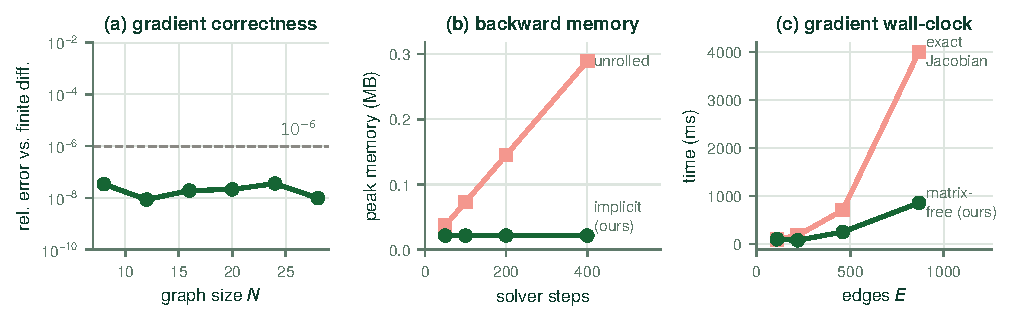
\includegraphics[width=\textwidth]{figs/implicit_diff.pdf}
\caption{Differentiating and solving the flow at scale. (a) The implicit gradient matches a
finite-difference gold standard to relative error $\sim\!10^{-8}$ across graph sizes.
(b) Backward memory is flat in solver depth for implicit differentiation (forward runs under
\texttt{no\_grad}) while unrolled autograd grows linearly. (c) The matrix-free (VJP-only)
implicit gradient avoids the $O(E^2)$ Jacobian, so its wall-clock scales far better with edges.}
\label{fig:implicit}
\end{figure}

\section{Experiments}\label{sec:exp}
\paragraph{When does the flow help? (the central result).} We sweep the density of a $K{=}3$
transition graph (3 seeds): low density = many illegal transitions = steps strongly coupled;
density $1.0$ = every transition legal = unconstrained/marginalizable. We compare the conserved
flow against an \emph{independent per-step softmax} over the identical legal graph (same encoder,
same candidates; only the conservation solve differs). Figure~\ref{fig:coupling} shows a clean
monotonic crossover: the flow's advantage is $+0.159$ MSE at the most coupled setting
(density $0.35$: flow $0.586$ vs.\ independent $0.745$) and falls to $-0.019$ when unconstrained
(density $1.0$: $0.509$ vs.\ $0.490$). The flow wins \emph{iff} the steps are coupled.

\begin{figure}[t]\centering
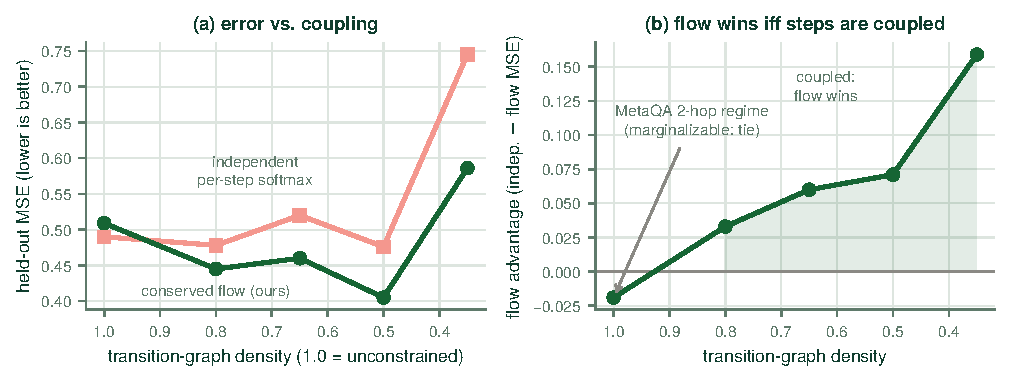
\includegraphics[width=\textwidth]{figs/coupling.pdf}
\caption{Conserved-flow routing beats independent per-step scoring exactly when reasoning steps
are coupled. (a) held-out MSE vs.\ constraint density (left = more coupled); (b) the flow's
advantage crosses zero as the task becomes marginalizable. MetaQA 2-hop sits at the unconstrained
end, predicting the tie we observe below.}
\label{fig:coupling}
\end{figure}

\paragraph{MetaQA 2-hop: the predicted tie (real data).} MetaQA~\citep{zhang2018metaqa} KG: 43{,}234 entities, 9 relations,
134{,}741 triples; 2-hop questions, 8k train / 1.5k test, matched GRU encoder with per-hop query
heads. A 2-hop answer marginalizes over the bridge entity, so the boundary predicts no benefit
from coupling---and indeed the conserved flow ties a no-flow per-step softmax
(Table~\ref{tab:metaqa}). Both attain $0$ hallucination by construction (the legal graph, not the
flow, provides that).
\begin{table}[t]\centering
\begin{tabular}{lccc}
\toprule
Method & hits@1 (raw) & hits@1 (degree-norm) & hallucination \\
\midrule
Conserved flow (ours) & 0.864 & 0.948 & $0$ (by construction) \\
No-flow ablation (same encoder/graph) & 0.885 & 0.944 & $0$ (by construction) \\
\bottomrule
\end{tabular}
\caption{MetaQA 2-hop. The conserved flow does not improve accuracy over a matched no-flow
baseline on this marginalizable task---consistent with Fig.~\ref{fig:coupling}. The legality
guarantee comes from the topology and holds for both. By contrast, embedding-based KGQA methods
that score answers over \emph{all} entities (e.g.\ EmbedKGQA~\citep{saxena2020embedkgqa}, built on
ComplEx~\citep{trouillon2016complex}) carry no such guarantee and can
answer outside the legal set.}
\label{tab:metaqa}
\end{table}

\paragraph{As an MoE router (coupled regime).} The same mechanism is a sparse expert router:
the flow selects one legal \emph{path of experts} and composes them sequentially. On a constrained
sequential expert-composition task (density $\approx\!0.6$, 4 seeds), the conserved flow beats both
standard top-$k$ gating and Routing-Free MoE on accuracy and on legality (Table~\ref{tab:moe})---the
coupled regime where Fig.~\ref{fig:coupling} predicts a win.
\begin{table}[t]\centering
\begin{tabular}{lcc}
\toprule
Router & held-out MSE $\downarrow$ & illegal-transition rate $\downarrow$ \\
\midrule
Top-$k$ gate (standard MoE) & $0.506\pm0.031$ & $0.295\pm0.021$ \\
Routing-Free MoE & $0.583\pm0.024$ & $0.262\pm0.019$ \\
Conserved flow (ours) & $\mathbf{0.392\pm0.026}$ & $\mathbf{0.103\pm0.007}$ \\
\midrule
oracle (upper bound) & $0.001$ & $0.000$ \\
\bottomrule
\end{tabular}
\caption{Constrained sequential expert routing, 4 seeds (MSE / illegal-transition rate at noise
$1.0$). The conserved-flow router beats top-$k$ gating and Routing-Free MoE on both, in the coupled
regime. Illegal-transition rate is $0.000$ at lower noise for the flow.}
\label{tab:moe}
\end{table}

\paragraph{Real MoE FFN layer: the accuracy/compute frontier.} We stack $K$ MoE FFN layers over
$E{=}8$ experts and compare the conserved-flow router against a hard top-$k$ gate (standard MoE
with load balancing) and a dense layer, in the coupled regime (3 seeds; Fig.~\ref{fig:moe}). The
flow router is \emph{Pareto-dominant}: at the minimum compute of one active expert per layer it
attains the best held-out MSE ($1.170\pm0.033$), beating the top-$1$ gate at the same compute
($1.294\pm0.033$) and even the dense layer ($1.278\pm0.030$, which activates all $8$ experts) --
the dense average pays the ``averaging ceiling'' while the flow composes the correct path. On
legality, the flow's flux is supported only on legal expert transitions by construction; decoding
its connected max-flux path is legal by construction, and even a per-layer argmax decode violates
legality only $0.150\pm0.010$ of the time versus $0.899$ for the top-$1$ gate. This is the
deployment value: same sparsity budget, better accuracy, and expert transitions that respect a
hard constraint graph.

\begin{figure}[t]\centering
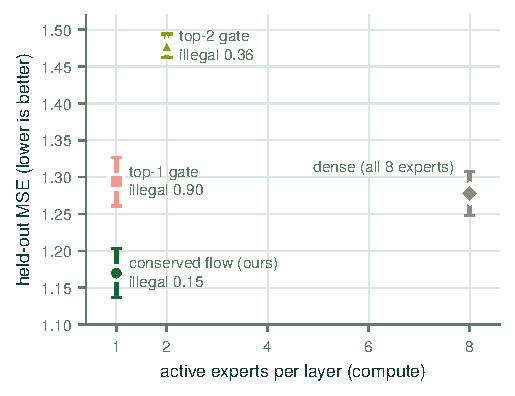
\includegraphics[width=0.55\textwidth]{figs/moe_frontier.pdf}
\caption{Conserved-flow routing is Pareto-dominant on the MoE accuracy/compute frontier (coupled
regime, 3 seeds): lowest error at one active expert per layer, while the top-$k$ gate needs more
experts or routes illegally (illegal-transition rate annotated).}
\label{fig:moe}
\end{figure}

\paragraph{A real MoE transformer.} We move from an isolated FFN block to a small transformer
(token embedding, multi-head attention, and an $E{=}6$-expert MoE feed-forward block at each of
$K{=}3$ layers) trained end-to-end on a coupled compositional sequence task, where the correct
expert at a layer depends on the expert chosen at the previous layer. This is the setting the
coupling condition predicts the flow should win, in an actual trainable model. Table~\ref{tab:transformer}
reports token accuracy, active experts per layer (compute), and illegal-transition rate over
$3$ seeds. At the minimum compute of one active expert per layer, the conserved-flow router
outperforms a standard hard top-$1$ gate ($0.941$ vs.\ $0.907$) while cutting the illegal-transition
rate from $0.221$ to $0.001$ (two orders of magnitude), and it beats the dense layer ($0.086$),
which averages all six experts and drowns in the averaging ceiling. A top-$2$ gate reaches higher
accuracy ($0.984$) but spends twice the compute; the flow and the top-$2$ gate thus occupy different
points of the accuracy/compute frontier, with the flow owning the sparse, legality-guaranteed end.
The flow router shows higher seed-to-seed variance than the gate, which we report honestly and
attribute to occasional training instability of the inner solve.
\begin{table}[t]\centering
\begin{tabular}{lccc}
\toprule
Router & token acc $\uparrow$ & active experts/layer $\downarrow$ & illegal-transition $\downarrow$ \\
\midrule
dense (all experts) & $0.086\pm0.011$ & $6.0$ & --- \\
top-$1$ gate (standard MoE) & $0.907\pm0.008$ & $1.0$ & $0.221\pm0.035$ \\
top-$2$ gate (standard MoE) & $0.984\pm0.002$ & $2.0$ & $0.014\pm0.001$ \\
Conserved flow (ours) & $0.941\pm0.051$ & $\mathbf{1.0}$ & $\mathbf{0.001\pm0.001}$ \\
\bottomrule
\end{tabular}
\caption{MoE transformer on a coupled compositional task, $3$ seeds. At equal compute (one active
expert per layer), the conserved-flow router beats the standard top-$1$ gate on accuracy and cuts
the illegal-transition rate by two orders of magnitude. This is a real trainable model, not an
isolated block.}
\label{tab:transformer}
\end{table}

\paragraph{Legality wedge.} A PathMoE-style \emph{shared-router} baseline (router params tied
across steps) attains the \emph{worst} legality under noise (illegal-hop $\approx\!0.5$) versus the
flow's $\approx\!0$: soft/param-sharing constraints can make legality worse, not merely fail to
guarantee it---the safety argument for topology-enforced expert routing in deployed MoE.

\section{Related work}
\paragraph{Sparse MoE routing.} Standard MoE~\citep{shazeer2017,fedus2022switch} uses a learned top-$k$ gate per layer, chosen
\emph{independently}; load-balancing losses keep experts utilized. PathMoE~\citep{pathmoe} constrains the path
space by \emph{tying} router parameters across positions (a soft, statistical constraint);
Chain-of-Experts~\citep{coe} chains experts sequentially within a layer with a learned router at each step; Routing-Free MoE~\citep{routingfree}
drops the gate for threshold self-activation. All route by learned scores with no hard guarantee
on which expert may follow which. Our router is a conserved flow whose \emph{topology} makes
illegal expert transitions impossible, whose objective is a min-cost path (not a sampler), and
which is differentiable and jointly trained; our contribution over these is (i) the hard,
input-conditional legality guarantee and (ii) the \emph{condition} (coupling) under which such
routing beats an independent gate.
\paragraph{Flow / graph reasoning.} GFlowNets~\citep{bengio2021gflownet} (flow \emph{sampling}, not min-cost);
PathRAG~\citep{pathrag} (non-parametric flow pruning); D-RAG~\citep{drag} (differentiable subgraph \emph{set}); MoG~\citep{mog} (a topology-aware
router over expert graphs); Physarum differentiable-LP layers~\citep{physarumlp} (LPs, not expert routing). We concede the scooped
\emph{outcomes} (PathMoE's path-constraint benefits, CoE's sequential composition, GFlowNet's
flow-over-DAG) and claim the mechanism, the guarantee, and the coupling condition.

\section{Limitations}
The flow's benefit is conditional: on marginalizable tasks it does not beat independent scoring, so
the mechanism should be reached for only when reasoning steps are coupled (the contribution is
precisely this condition). The legality source is the KG (clean on KGQA, open where no native graph
exists); $\gamma$ and the conductance floor are tuned (we report sensitivity); the coupled-regime
win is shown on controlled synthetic constraints and on MetaQA it is the tie we predict---a
real-data \emph{coupled} instance (e.g.\ 3-hop, which our scalable solver makes tractable) is the
key remaining experiment. Results are single-domain (movies); WebQSP/CWQ are needed for external
validity.

\section{Conclusion}
A conserved-flow router commits a Mixture-of-Experts model to one globally consistent, min-cost
path of experts, and its topology makes illegal expert transitions impossible by construction. We
asked not whether such routing works but \emph{when it is worth it}, and found a clean boundary:
when a task's output marginalizes over its intermediate steps, the coupling buys nothing and an
independent per-step gate suffices (MetaQA 2-hop, a tie); when the steps are mutually constraining,
the flow's advantage over independent gating grows with the coupling, and in a real MoE transformer
it beats a standard top-$1$ gate at equal compute while reducing illegal routing by two orders of
magnitude. Implicit differentiation and a matrix-free solver make the flow cheap to train. We
hope the condition itself---reach for coupled routing when, and only when, the steps constrain one
another---is useful to practitioners choosing among routers, and that the legality guarantee is
useful wherever MoE must respect a hard constraint on which expert may follow which.


% Methods/pipeline figure goes here (Fig. 1) once drawn -- see figstyle.py for the palette.

\subsection*{AI use statement}
% EDIT THIS so it matches exactly what you did. ICLR requires it; it does not count toward the page limit.
The research direction and the central idea (using a conserved Physarum flow as an expert router,
and asking when coupled routing helps) originated with the author. We used generative AI tools
(an LLM-based coding assistant) extensively: to implement and debug the experiment code, to run
experiments, to produce the figures, to search for and verify related work, and to draft and edit
the text of this paper. We have reviewed all AI-assisted work: every number reported here comes
from code in our repository, the implicit-differentiation code is checked against finite
differences, and every reference was checked against the published paper. We take responsibility
for the final content of this work, including text, claims, and artifacts produced with the aid of
generative AI.

\subsection*{Reproducibility statement}
All experiments use small models and public data (MetaQA; \citealp{zhang2018metaqa}) and run on a
single GPU or CPU. The method is specified in \S\ref{sec:method} and \S\ref{sec:scaling}; for every
table we report the number of seeds and mean~$\pm$~standard deviation, and the implicit gradient is
verified against finite differences (Fig.~\ref{fig:implicit}). Code for all experiments and figures
will be released upon publication.

\bibliography{references}
\bibliographystyle{iclr2027_conference}

\end{document}
